\documentclass[12pt]{article}
\usepackage[utf8]{inputenc} 
\usepackage{ dsfont }

\usepackage{ amssymb }
\usepackage{amsfonts}
\usepackage{algorithm}
\usepackage{amsmath}
\usepackage{algpseudocode}
\usepackage{graphicx}
\usepackage{tikz} %Рисование автоматов
\usetikzlibrary{automata,positioning,shapes,snakes,arrows}
\usetikzlibrary{arrows}
\usepackage[english,russian]{babel}
\usepackage{hyperref}
\usepackage{ upgreek }
\usepackage{colortbl}

\definecolor{urlcolor}{HTML}{799B03}

\hypersetup{pdfstartview=FitH,  urlcolor=urlcolor, colorlinks=true}
\title{Lab work 7\\ 4D-video dimensionality reduction}

\date{}
\author{Pankratov Viktor} 
\begin{document}
\maketitle
\selectlanguage{english}
\tableofcontents
\newpage
\section{Lab 7 report}

\subsection{Motivation}
Data in computer vision is often characterised by plotting into less-dimensional subspaces using algorithms such as PCA or PLS. Every element is supposed to be vector, not tensor or even 2-dimensional matrix. However, one of the data types is video and there exist videos in even more than 3-dimensional space. To be able to project such videos to more comfortable less-dimensional spaces HOPCA is proposed.
\subsection{Problem statement}
Given a sequence of images $\{\upchi_i\}_{i=1}^{T}$, every image is a 4-dimensional tensor containing integer values. Thus video is a 5-dimensional tensor with first four axes coordinates representing the position of pixel in 4d-space and the fifth representing time.
$$\upchi \in R^{D_1 \times D_2 \times D_3 \times D_4} \times T $$ The goal is to make a compact video representation by reducing its dimensions.
\subsection{Solution}
It is supposed to use PCA with tensor notation. PCA is a method which involves SVD of the data matrix $X$.
$$X = USV^T = U^{(1)}SU^{(2)} = S \times_1 U^{(1)} \times_2 U^{(2)}$$
Then the basic vectors are columns of $U^{(1)}$ and the coordinates in that basic are defined by $SU^{(2)^T}$ \\
HOPCA is a direct PCA extension to multilinear case. In particular that means that HOPCA with vector samples is equivalent to PCA. Otherwise tensor $\upchi$ is decomposed:
$$\upchi = S \times_1 U^{(1)} \times_2 \dots \times_n U^{(n)} $$ 
As in SVD, HOSVD keeps first columns for each $U^{(i)}$ to produce $\hat{U}^{(i)}$and input tensor $Z$ is projected to a lower dimensional tensor as
$$Y = Z \times \hat{U}^{(1)^T} \times \dots$$
\subsection{Experimental results}
For experimental simplicity every image tensor contains boolean values. Simple sequences of images were generated, one of projections of which onto 3-dimensional space are shown below.For multidimensional case they are mixed into one bicolor image:one of them is responsible for blue color and one of them for green.\\
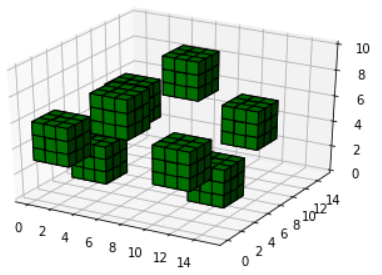
\includegraphics[scale=0.8]{1.png}
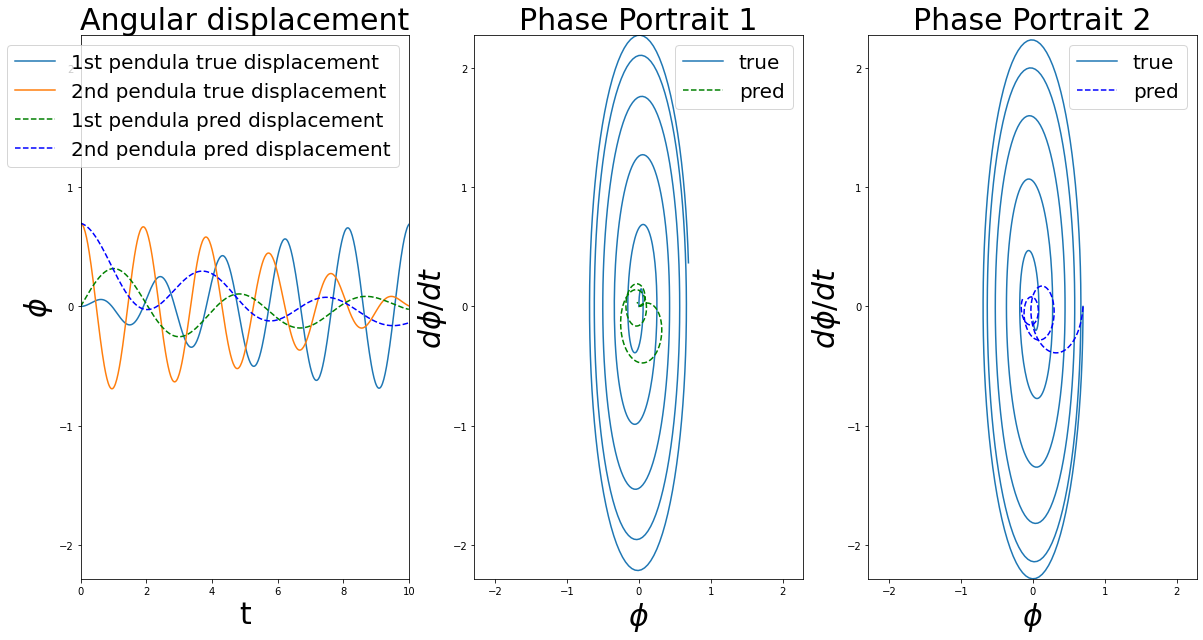
\includegraphics[scale=0.8]{2.png}
\\
Cube transformation using using PCA.\\
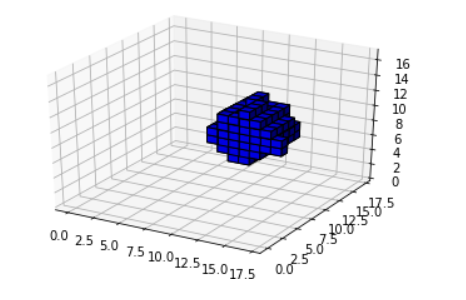
\includegraphics[scale=0.8]{4.png}\\
That experiment was just for demonstration how the 4-dimensional cube will look like after PCA transformation. 

\newpage
Bicolor image transformation using HOPCA.\\
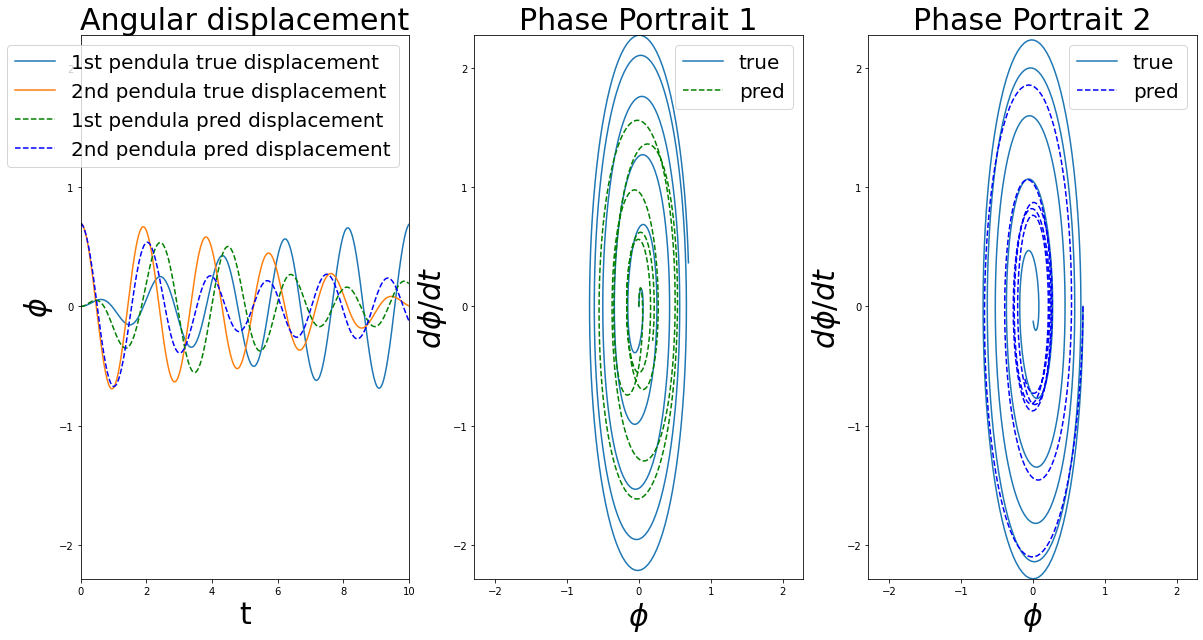
\includegraphics[scale=0.8]{3.png}\\
During the generation process the original cube coordinates were taken mod 15 where 15 is the image one coordinate size. A cube dividing into several areas was expected. As we can see, there are 3 colors: blue, green and black.
\par 
Considering binary images one of the blue and green colors has to disappear. After PCA one of their color values is strictly less than 
background and one of them is strictly more. Either blue or green color would be combined with background.
\par 
Considering gray-scale images blue and green cubes remain. Still there are black cubes which meaning is intersection of previous two. And after transformation their color values are almost equal to background. That means that in this example after projection any information about intersection is lost and HOPCA might be not fit for the problem.   
\subsection{Useful links}
The MPCA implementation was taken from the following \href{https://www.mathworks.com/matlabcentral/fileexchange/26168-multilinear-principal-component-analysis-mpca?s_tid=mwa_osa_a}{link}. Other parts of the code are available on \href{https://github.com/PankratovViktor/MMP_Lab1}{Github}
\begin{itemize}
\item[1]{Tucker Tensor Decomposition on FPGA.
Kaiqi Zhang, Xiyuan Zhang, Zheng Zhang}
\item[2]{J. Yang, D. Zhang, A. F. Frangi, and J. Yang. Twodimensional pca: a new approach to appearance-based face
representation and recognition}
\item[3]{Multilinear Principal Component Analysis of Tensor Objects for Recognition.
Haiping Lu, K.N. Plataniotis and A.N. Venetsanopoulos
}
\end{itemize}
\end{document}